\documentclass{article}
\usepackage[utf8]{inputenc}
\usepackage{enumitem}
\usepackage{ulem}
\usepackage{mathrsfs}
\usepackage{amsmath}
\usepackage{float}
\usepackage{hyperref}
\usepackage{xcolor}
\usepackage{listings}
\usepackage{color}
\usepackage[utf8]{inputenc}
\usepackage{CJK}
\usepackage{amsthm,amsmath,amssymb}
\usepackage{hyperref}
\usepackage{relsize}
\usepackage{graphicx}
\usepackage{bbm}

\newtheorem{problem}{Problem}

\newcommand{\N}{\mathcal N}
\newcommand{\Y}{\mathbf Y}
\newcommand{\real}{\mathbb{R}}
\newcommand{\X}{\mathbf X}
\newcommand{\Z}{\mathbf Z}

\newcommand*{\tran}{^{\mkern-1.5mu\mathsf{T}}}
\newcommand*{\hermitian}{^{\mkern-1.5mu\mathsf{H}}}

\newcommand{\Tau}{\mathrm{T}}

\DeclareMathOperator{\Tr}{Tr}

\def\Epsilon{E}
\def\Eta{H}

\def\veczero{{\mathbf 0}}
\def\vec1{{\mathbf 1}}
\def\matzero{{\mathbf 0}}

\def\veca{{\mathbf a}}
\def\vecb{{\mathbf b}}
\def\vecc{{\mathbf c}}
\def\vecd{{\mathbf d}}
\def\vece{{\mathbf e}}
\def\vecf{{\mathbf f}}
\def\vecg{{\mathbf g}}
\def\vech{{\mathbf h}}
\def\veck{{\mathbf k}}
\def\vecm{{\mathbf m}}
\def\vecn{{\mathbf n}}
\def\vecp{{\mathbf p}}
\def\vecq{{\mathbf q}}
\def\vecr{{\mathbf r}}
\def\vect{{\mathbf t}}
\def\vecu{{\mathbf u}}
\def\vecv{{\mathbf v}}
\def\vecw{{\mathbf w}}
\def\vecx{{\mathbf x}}
\def\vecy{{\mathbf y}}
\def\vecz{{\mathbf z}}

\def\vecalpha{{\mathbf \alpha}}
\def\vecbeta{{\mathbf \beta}}
\def\vecepsilon{{\boldsymbol \epsilon}}
\def\veclambda{{\mathbf \lambda}}
\def\vecvarepsilon{{\boldsymbol \varepsilon}}
\def\vecgamma{{\boldsymbol \gamma}}
\def\vecmu{{\boldsymbol \mu}}
\def\vecnu{{\boldsymbol \nu}}
\def\vecomega{{\boldsymbol \omega}}
\def\vecphi{{\boldsymbol \phi}}
\def\vecpsi{{\boldsymbol \psi}}
\def\vecsigma{{\mathbf \sigma}}
\def\vecvarsigma{{\mathbf \varsigma}}
\def\vectau{{\boldsymbol \tau}}
\def\vecupsilon{{\boldsymbol \upsilon}}
\def\vecvarphi{{\boldsymbol \varphi}}
\def\vecxi{{\boldsymbol \xi}}
\def\veczeta{{\boldsymbol \zeta}}


\def\vecX{{\mathbf X}}
\def\vecY{{\mathbf Y}}
\def\vecZ{{\mathbf Z}}

\def\vecEpsilon{{\mathbf \Epsilon}}
\def\vecEta{{\mathbf \Eta}}


\def\matA{{\mathbf A}}
\def\matB{{\mathbf B}}
\def\matC{{\mathbf C}}
\def\matD{{\mathbf D}}
\def\matE{{\mathbf E}}
\def\matF{{\mathbf F}}
\def\matH{{\mathbf H}}
\def\matI{{\mathbf I}}
\def\matK{{\mathbf K}}
\def\matL{{\mathbf L}}
\def\matO{{\mathbf O}}
\def\matOmega{{\mathbf \Omega}}
\def\matN{{\mathbf N}}
\def\matP{{\mathbf P}}
\def\matS{{\mathbf S}}
\def\matU{{\mathbf U}}
\def\matV{{\mathbf V}}
\def\matW{{\mathbf W}}
\def\matX{{\mathbf X}}
\def\matZ{{\mathbf Z}}
\def\matGamma{{\mathbf{\mathrm{\Gamma}}}}
\def\matLambda{{\mathbf{\mathrm{\Lambda}}}}
\def\matOmega{{\mathbf{\mathrm{\Omega}}}}
\def\matPhi{{\mathbf \Phi}}
\def\matPsi{{\mathbf \Psi}}
\def\matRho{{\mathbf{\mathrm{P}}}}
\def\matSigma{{\mathbf{\mathrm{\Sigma}}}}
\def\matUpsilon{{\mathbf{\mathrm{\Upsilon}}}}
\def\matXi{{\mathbf{\mathrm{\Xi}}}}

\def\matzero{{\mathbf 0}}


\def\complex{{\mathbb {C}}}
\def\real{{\mathbb {R}}}
\def\extreal{\overline{\mathbb {R}}}
\def\rational{{\mathbb {Q}}}
\def\pnint{{\mathbb {Z}}}
\def\nnint{{\mathbb{N}_0}}
\def\pint{{\mathbb {N}}}
\def\extint{\overline{\mathbb {Z}}}

\def\defas{:=}
\def\as{\overset{\mbox{a.s.}}{=}}
\def\ind{1}
\def\normal{\calN}
\def\expect{\mathbb{E}}
\def\variance{\mbox{Var}}
\def\covariance{\mbox{Cov}}
\def\prob{\mathbb{P}}
\def\risk{\calR}
\def\Uniform{{\cal{U}}}
\def\Trace{\mbox{Tr}}
\def\sign{\mbox{sign}}
\def\evaloss{\star}
\def\margin{\varrho}
\def\Log{{Log}}

\def\converged{\xrightarrow[]{D}}
\def\convergep{\xrightarrow[]{P}}
\def\convergeas{\xrightarrow[]{a.s.}}

\def\Borel{{\frakB}}

\def\Re{\mbox{Re}}
\def\Im{\mbox{Im}}

\def\interior{\mathrm{o}}

\def\calA{{\cal A}}
\def\calB{{\cal B}}
\def\calC{{\cal C}}
\def\calD{{\cal D}}
\def\calE{{\cal E}}
\def\calF{{\cal F}}
\def\calG{{\cal G}}
\def\calH{{\cal H}}
\def\calK{{\cal K}}
\def\calL{{\cal L}}
\def\calM{{\cal M}}
\def\calN{{\cal N}}
\def\calP{{\cal P}}
\def\calR{{\cal R}}
\def\calS{{\cal S}}
\def\calT{{\cal T}}
\def\calV{{\cal V}}
\def\calX{{\cal X}}
\def\calY{{\cal Y}}
\def\calZ{{\cal Z}}

\def\scrA{\mathscr{A}}
\def\scrB{\mathscr{B}}
\def\scrC{\mathscr{C}}
\def\scrD{\mathscr{D}}
\def\scrE{\mathscr{E}}
\def\scrF{\mathscr{F}}
\def\scrG{\mathscr{G}}
\def\scrI{\mathscr{I}}
\def\scrJ{\mathscr{J}}
\def\scrK{\mathscr{K}}
\def\scrL{\mathscr{L}}
\def\scrM{\mathscr{M}}
\def\scrN{\mathscr{N}}
\def\scrP{\mathscr{P}}
\def\scrQ{\mathscr{Q}}
\def\scrR{\mathscr{R}}
\def\scrS{\mathscr{S}}
\def\scrU{\mathscr{U}}
\def\scrV{\mathscr{V}}
\def\scrX{\mathscr{X}}


\def\pzch{\mathpzc{h}}
\def\pzcy{\mathpzc{y}}

\def\frakA{\mathfrak{A}}
\def\frakB{\mathfrak{B}}
\def\frakG{\mathfrak{G}}
\def\frakM{\mathfrak{M}}

\def\continuous{{\cal C}}


\addtolength{\oddsidemargin}{-.875in}
\addtolength{\evensidemargin}{-.875in}
\addtolength{\textwidth}{1.75in}
\addtolength{\topmargin}{-.875in}
\addtolength{\textheight}{1.75in}

\title{ML2023 Fall Homework Assignment 1\\ Handwritten}
\author{Lecturor: Pei-Yuan Wu\\
TAs: \textcolor{red}{Yuan-Chia Chang, Chun-Lin Huang}}
\date{Sep 2023}

\begin{document}

\maketitle



\section*{Problem 1 (Preliminary) (1 pt)}
\begin{enumerate}
    \item[(a)] (0.2 pts) Given $\vecw\in \real^m$,  $\matA\in\mathbb{R}^{m\times m}$. Show that
    $$\nabla_\vecw \vecw\tran \matA\mathbf{w} = \matA\tran \vecw + \matA\vecw.$$
    In particular, if $\matA$ is a symmetric matrix, then
    $$\nabla_\vecw \vecw\tran \matA\mathbf{w} = 2\matA\vecw$$
    %
    \item[(b)] (0.2 pts) Given $\matA, \matB \in \real^{m \times m}$. Show that
    \begin{equation}\label{eq:matrix_product_trace_derivative}
    \frac{\partial\ tr(\matA\matB)}{\partial a_{ij}} = b_{ji}
    \end{equation}
    where
    \begin{equation*}
    \matA=\left[\begin{array}{cccc}
    a_{11} & a_{12} & \cdots & a_{1 m} \\
    a_{21} & a_{22} & \cdots & a_{2 m} \\
    \vdots & \vdots & \ddots & \vdots \\
    a_{m 1} & a_{m 2} & \cdots & a_{m m}
    \end{array}\right], ~~
    \matB=\left[\begin{array}{cccc}
    b_{11} & b_{12} & \cdots & b_{1 m} \\
    b_{21} & b_{22} & \cdots & b_{2 m} \\
    \vdots & \vdots & \ddots & \vdots \\
    b_{m 1} & b_{m 2} & \cdots & b_{m m}
    \end{array}\right]
    \end{equation*}
    %
    It is common to write (\ref{eq:matrix_product_trace_derivative}) as     
    $$\frac{\partial\ tr(\matA\matB)}{\partial \matA} = \matB\tran.$$
    %
    \item[(c)] (0.6 pts) Prove that
    \begin{equation}\label{eq:matrix_det_log_derivative}
    \frac{\partial \log(\det(\boldsymbol{\matA}))}{\partial a_{ij}} =  \vece_j\tran \boldsymbol{\matA}^{-1}\space \vece_i,
    \end{equation}
    %
    where $\boldsymbol{\matA} = \left[\begin{array}{cccc}
    a_{11} & a_{12} & \cdots & a_{1 m} \\
    a_{21} & a_{22} & \cdots & a_{2 m} \\
    \vdots & \vdots & \ddots & \vdots \\
    a_{m 1} & a_{m 2} & \cdots & a_{m m}
    \end{array}\right]
     \in \real^{m\times m}$ is a (non-singular) matrix, and $\mathbf{e}_j$ is the unit vector along the j-th axis (e.g. $\mathbf{e}_3=[0,0,1,0,...,0]^T$).
     It is common to write (\ref{eq:matrix_det_log_derivative}) as
     $$\frac{\partial \log(\det(\matA))}{\partial \matA} =  \left(\matA^{-1}\right)\tran$$
\end{enumerate}

\section*{Problem 1 ans}
\begin{enumerate}[label=(\alph*)]
    \item Conseider $f(\mathbf{w}) = \mathbf{w}^T A \mathbf{w}$, and $f(\mathbf{w}+h) = (\mathbf{w} + h)^T A (\mathbf{w} + h)$
    Then, 
    $$
    \begin{aligned}
    f(\mathbf{w}+h) - f(\mathbf{w}) &=  \mathbf{w}^T A\mathbf{w} + h^T A \mathbf{w} + \mathbf{w}^TA h + h^T A h -  \mathbf{w}^T A \mathbf{w}\\
    &= h^T A \mathbf{w} + \mathbf{w}^TA h + h^T A h\\
    &= h^T(A^T \mathbf{w} + A\mathbf{w}) + h^T A h\\
    &= (A^T \mathbf{w} + A\mathbf{w})\cdot h + h^T A h
    \end{aligned}
    $$
    By definition, $\frac{\partial\ \mathbf{w}^TA\mathbf{w}}{\partial\ \mathbf{w}} = A^T\mathbf{w} + A\mathbf{w}$. In particular, $A$ is a symmetric matrix i.e. $A = A^T$, then $\frac{\partial\ \mathbf{w}^TA\mathbf{w}}{\partial\ \mathbf{w}} = 2A\mathbf{w}$
    \item Define $C = AB$. Note that $c_{ij} := \sum_{k=1}^m a_{ik}b_{kj}$, where $c_{ij}$ is the $i$-th row and $j$-th columns of matrix $C$. i.e. the dot product of the $i$-th row of $A$ and the $j$-th column of $B$.
    Then, 
    $$
    tr(AB) = tr(C) = \sum_{l=1}^m c_{ll} = \sum_{l=1}^m\sum_{k=1}^m a_{lk}b_{kl}
    $$
    Hence, 
    $$
    \begin{aligned}
    \frac{\partial\ tr(AB)}{\partial a_{ij}} &= \frac{\partial\ \sum_{l=1}^m\sum_{k=1}^m a_{lk}b_{kl}}{\partial a_{ij}} =b_{ji}
    \end{aligned}
    $$
    \item Follow the hint
    \begin{figure}[h]
         \centering
         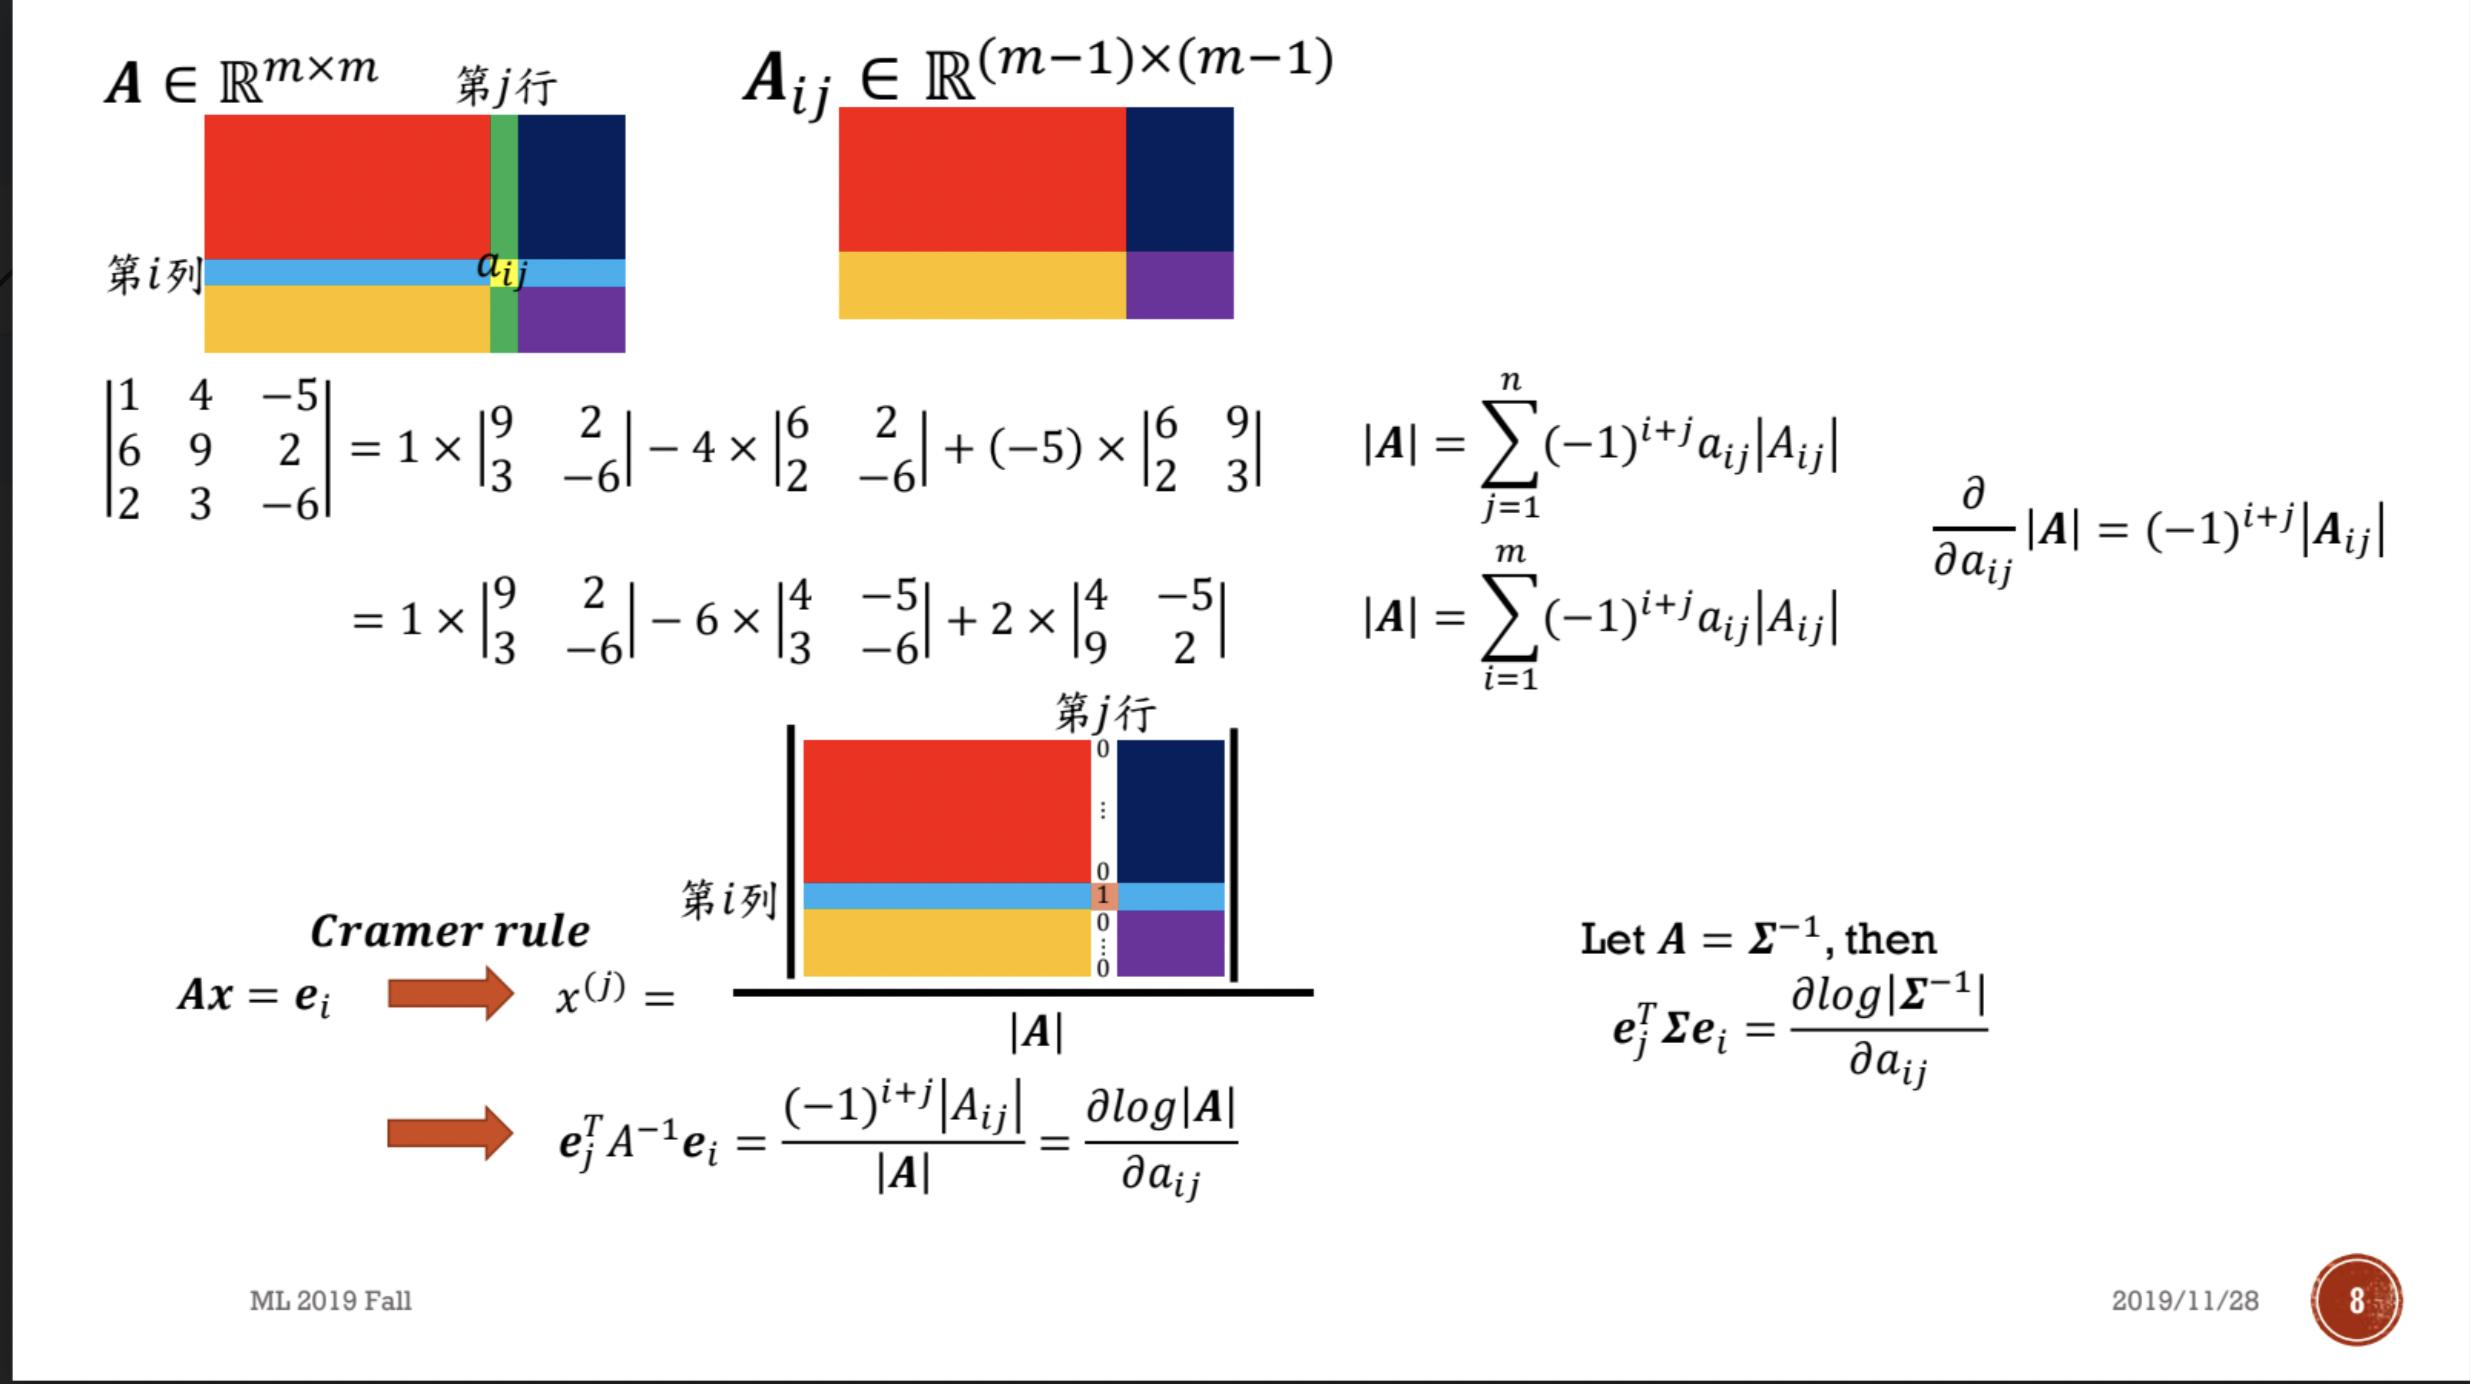
\includegraphics[width=0.8\textwidth]{hint.jpg}
     \end{figure}
\end{enumerate}


\section*{Problem 2 (Classification with Gaussian Mixture Model) (2.4 pts)}

In this question, we tackle the binary classification problem through the generative approach, where we assume the data point $X$ (viewed as a $\real^d$-valued r.v.) and its label $Y$ (viewed as a $\{\calC_1,\calC_2\}$-valued r.v.) are generated according to the generative model (paramerized by $\theta$) as follows:
\begin{equation}\label{eq:two_gaussian}
\prob_\theta [X = \vecx,Y = \calC_k] = \pi_k f_{\vecmu_k,\matSigma_k}(\vecx)~~ (k \in \{1,2\})
\end{equation}
%
where $\theta = (\pi_1,\pi_2,\vecmu_1,\vecmu_2,\matSigma_1,\matSigma_2)$ for which
\begin{equation*}
f_{\vecmu_k,\matSigma_k}(\vecx) = \frac{1}{(2\pi)^{d/2}}\frac{1}{\left| \matSigma_k \right|^{1/2}}\exp\left(-\frac{1}{2}(\vecx-\vecmu_k)\tran \matSigma_k^{-1}(\vecx-\vecmu_k)\right).
\end{equation*}
%
Now suppose we observe data points $\vecx_1,...,\vecx_N$ and their corresponding labels $y_1,...,y_N$.
\begin{enumerate}[label=(\alph*)]
\item (1.2 pt)
\begin{enumerate}[label=(\roman*)]
\item (0.3 pt) Please write down the likelihood function $L(\theta)$ that describes how likely the generative model would generate the observed data $\{(\vecx_i,y_i)\}_{i=1}^N$ in terms of $\theta = (\pi_1,\pi_2,\vecmu_1,\vecmu_2,\matSigma_1,\matSigma_2)$.
%
\item (0.3 pt) Find the maximum likelihood estimate $\theta^* = (\pi^*_1,\pi^*_2,\vecmu^*_1,\vecmu^*_2,\matSigma^*_1,\matSigma^*_2)$ that maximizes the likelihood function $L(\theta)$. %(Note that we do not assume $(\Sigma_1^*,\Sigma_2^*)$ are the same)
%
\item (0.3 pt) Write down $\prob_\theta[Y=\calC_1|X=\vecx]$ and $\prob_\theta[X=\vecx|Y=\calC_1]$ in terms of $\theta = (\pi_1,\pi_2,\vecmu_1,\vecmu_2,\matSigma_1,\matSigma_2)$. What are the physical meaning of the aforementioned quantities?
%
\item (0.3 pt) Express $\prob_\theta[Y=\calC_1|X=\vecx]$ in the form of $\sigma(z)$, where $\sigma(\cdot)$ denotes the sigmoid function, and express $z$ in terms of $\theta = (\pi_1,\pi_2,\vecmu_1,\vecmu_2,\matSigma_1,\matSigma_2)$ and $x$.
\end{enumerate}
%
\item (1.2 pt) Suppose we pose an additional constraint that the covariance matrices of the two Gaussian distributions are identical, namely $\Sigma_1=\Sigma_2=\Sigma$, in which the generative model is parameterized by $\vartheta = (\pi_1,\pi_2,\vecmu_1,\vecmu_2,\matSigma)$. Redo questions (a) under such setting.
\end{enumerate}

\section*{Problem 2 ans}
\begin{enumerate}[label=(\alph*)]
    \item
    \begin{enumerate}[label=(\roman*)]
        \item The likelihood function is given by
        \[
        L(\theta) = \prod_{i=1}^{N}(\mathbbm{1}(y_i=C_1)\pi_1 f_{\vecmu_1,\matSigma_1}(\vecx_i) + \mathbbm{1}(y_i=C_2)\pi_2 f_{\vecmu_2,\matSigma_2}(\vecx_i))
        \]
        Since the indicator function is not differentiable, you may write it in a another format.\\
        W.L.O.G we may assume that there are $N_1$ numbers of $y_i \in C_1$, $N_2$ numbers of $y_i \in C_2$ and $N_1+N_2=N$The likelihood function is given by
        \begin{align*}
        L(\theta) = &\frac{1}{(2\pi)^{dN/2}}\pi_1^{N_1}\pi_2^{N_2}\frac{1}{\left| \matSigma_1 \right|^{N_1/2}}\frac{1}{\left| \matSigma_2 \right|^{N_2/2}}\times\\
        &\prod_{i,y_i=C_1}^{N_1}\exp\left(-\frac{1}{2}(\vecx_i-\vecmu_1)\tran \matSigma_1^{-1}(\vecx_1-\vecmu_1)\right) \prod_{j,y_j=C_2}^{N_2}\exp\left(-\frac{1}{2}(\vecx_j-\vecmu_2)\tran \matSigma_2^{-1}(\vecx_j-\vecmu_2)\right)
        \end{align*}
        \item To make the calculation easier later, we change the above answer into log likelihood function
        \begin{align*}
        L-log(\theta) = &log(\frac{1}{(2\pi)^{dN/2}})+N_1log(\pi_1)+N_2log(\pi_2) +\frac{-N_1}{2}log(\left| \matSigma_1 \right|)+\frac{-N_2}{2}log(\left| \matSigma_2 \right|)+\\
        &\sum_{i,y_i=C_1}^{N_1}\left(-\frac{1}{2}(\vecx_i-\vecmu_1)\tran \matSigma_1^{-1}(\vecx_1-\vecmu_1)\right)+\sum_{j,y_j=C_2}^{N_2}\left(-\frac{1}{2}(\vecx_j-\vecmu_2)\tran\matSigma_2^{-1}(\vecx_j-\vecmu_2)\right)
        \end{align*}
        Now we calculate the optimal $\pi_1^*,\pi_2^*$. Note that $\pi_1+\pi_2=1$
        \begin{align*}
        \frac{\partial L-log(\theta)}{\partial \pi_1} &=\frac{N_1}{\pi_1} + \frac{N_2}{1-\pi_1}=0\\
        (1-\pi_1)N_1+\pi_1 N_2 =0& \Rightarrow \pi_1*=\frac{N_1}{N}
        \end{align*}
        same for $\pi_2$ we have \[\pi_2^*=\frac{N_2}{N}\]

        for $\mu_1^*,\mu_2^*$
        \begin{align*}
        \frac{\partial L-log(\theta)}{\partial \mu_1} &=\sum_{i,y_i=C_1}^{N_1}\left(\matSigma_1^{-1}(\vecx_1-\vecmu_1)\right)=\matSigma_1^{-1}\sum_{i,y_i=C_1}^{N_1}\left(\vecx_1-\vecmu_1\right)=0\\
        \sum_{i,y_i=C_1}^{N_1}\left(\vecx_1-\vecmu_1\right)=0& \Rightarrow \mu_1*=\frac{\sum_{i,y_i=C_1}^{N_1}x_i}{N_1}
        \end{align*}
        same for $\mu_2$ we have \[\mu_2^*=\frac{\sum_{i,y_i=C_2}^{N_2}x_i}{N_2}\]
        for  $\Sigma_1^*,\Sigma_2^*$, note that 
        \[
        \frac{\partial L-log(\theta)}{\partial \Sigma_1} = \frac{\partial L-log(\theta)}{\partial \Sigma_1^{-1}}\frac{\partial \Sigma_1^{-1}}{\partial \Sigma_1}=0
        \]
        Since the later one is not $0$. We need the former one to be $0$.
        \begin{align*}
        \frac{\partial L-log(\theta)}{\partial \Sigma_1^{-1}} &= \frac{1}{2}\frac{\partial-N_1log(\left| \matSigma_1 \right|)}{\partial \Sigma_1^{-1}} + \frac{\partial\sum_{i,y_i=C_1}^{N_1}\left(-\frac{1}{2}(\vecx_i-\vecmu_1)\tran \matSigma_1^{-1}(\vecx_i-\vecmu_1)\right)}{\partial \Sigma_1^{-1}}\\
        &=\frac{1}{2}\frac{\partial N_1log(\left| \matSigma_1^-1 \right|)}{\partial \Sigma_1^{-1}} + -\frac{1}{2}\frac{\partial\sum_{i,y_i=C_1}^{N_1}tr\left((\vecx_i-\vecmu_1)\tran \matSigma_1^{-1}(\vecx_i-\vecmu_1)\right)}{\partial \Sigma_1^{-1}}\\
        &=\frac{1}{2}\left( N_1\Sigma_1^T - \frac{\partial\sum_{i,y_i=C_1}^{N_1}tr\left(\matSigma_1^{-1}(\vecx_i-\vecmu_1)(\vecx_i-\vecmu_1)\tran \right)}{\partial \Sigma_1^{-1}}\right)\\
        &=\frac{1}{2}\left( N_1\Sigma_1^T - \sum_{i,y_i=C_1}^{N_1}(\vecx_i-\vecmu_1)(\vecx_i-\vecmu_1)\tran \right) = 0\\
        \left( N_1\Sigma_1^T - \sum_{i,y_i=C_1}^{N_1}(\vecx_i-\vecmu_1)(\vecx_i-\vecmu_1)\tran \right) = 0 & \Rightarrow \Sigma_1^*=\frac{\sum_{i,y_i=C_1}^{N_1}(\vecx_i-\vecmu_1)(\vecx_i-\vecmu_1)\tran}{N_1}
        \end{align*}
        same for $\Sigma_2$ we have \[\Sigma_2^*=\frac{\sum_{i,y_i=C_2}^{N_2}(\vecx_i-\vecmu_2)(\vecx_i-\vecmu_2)\tran}{N_2}\]
        \item $\prob_\theta[X=\vecx|Y=\calC_1]= \frac{\prob(X=x,Y=C_1)}{\prob(Y=C_1)}=f_{\vecmu_1,\matSigma_1}(\vecx)$ which means the probability of$x$ given the class \\
        $\prob_\theta[Y=\calC_1|X=\vecx] = \frac{\prob(X=x,Y=C_1)}{\prob(X=x)} = \frac{\pi_1f_{\vecmu_1,\matSigma_1}(\vecx)}{\pi_1f_{\vecmu_1,\matSigma_1}(\vecx)+\pi_2f_{\vecmu_2,\matSigma_2}(\vecx)}$ which means when we sample a new $x$ how likely is it belongs to $C_1$
        \item Same as the induction in class we have
        \[
        z = ln\frac{\left| \matSigma_2 \right|^{1/2}}{\left| \matSigma_1 \right|^{1/2}} - \frac{1}{2}x^t(\Sigma_1)^{-1}x + \mu_1^T(\Sigma_1)^{-1}x-\frac{1}{2}\mu_1^T(\Sigma_1)^{-1}\mu^1+\frac{1}{2}x^t(\Sigma_2)^{-1}x-\mu_2^T(\Sigma_2)^{-1}x+\frac{1}{2}\mu_2^T(\Sigma_2)^{-1}\mu_2+ln\frac{N_1}{N_2}
        \]
    \end{enumerate}
    \item we only show those are modified.
    \begin{enumerate}[label=(\roman*)]
        \item 
        \begin{align*}
        L(\theta) = &\frac{1}{(2\pi)^{dN/2}}\pi_1^{N_1}\pi_2^{N_2}\frac{1}{\left| \matSigma \right|^{N/2}}\\
        &\prod_{i,y_i=C_1}^{N_1}\exp\left(-\frac{1}{2}(\vecx_i-\vecmu_1)\tran \matSigma^{-1}(\vecx_1-\vecmu_1)\right) \prod_{j,y_j=C_2}^{N_2}\exp\left(-\frac{1}{2}(\vecx_j-\vecmu_2)\tran \matSigma^{-1}(\vecx_j-\vecmu_2)\right)
        \end{align*}
        \item 
        \[
        \Sigma^* = \frac{\sum_{i,y_i=C_1}^{N_1}(\vecx_i-\vecmu_1)(\vecx_i-\vecmu_1)\tran+\sum_{i,y_i=C_2}^{N_2}(\vecx_i-\vecmu_2)(\vecx_i-\vecmu_2)\tran}{N}
        \]
        \item the same
        \item 
        \[
        z = (\mu_1-\mu_2)^T\Sigma^{-1}x- \frac{1}{2}\mu_1^T(\Sigma_1)^{-1}\mu_1+ \frac{1}{2}\mu_2^T(\Sigma_1)^{-1}\mu_2 + ln\frac{N_1}{N_2}
        \]
    \end{enumerate}
\end{enumerate}

\section*{Problem 3 (Application of Gaussian Mixture Model Classifier) (0.6 pts)}
In this question, you will train a binary classifier based on the data which can be downloaded from \href{https://reurl.cc/2EZMzn}{https://reurl.cc/2EZMzn}  following the settings in Problem 2. Each data point and its label take the format $x_i \in \real^2$ and $y_i \in \{0,1\}$. 
\begin{enumerate}[label=(\alph*)]
    \item (0.2 pts) Calculate $\vartheta^* = (\pi^*_1,\pi^*_2,\vecmu^*_1,\vecmu^*_2,\matSigma^*)$ as in Problem 2 (b) in numbers.
    \item (0.2 pts) Calculate $\theta^* = (\pi^*_1,\pi^*_2,\vecmu^*_1,\vecmu^*_2,\matSigma^*_1,\matSigma^*_2)$ as in Problem 2 (a)(ii) in numbers.
    \item (0.2 pts) Please draw the scatter plot of the data. Which model is better in your opinion between (a) and (b)? Why?
\end{enumerate}

\section*{Problem 3 ans}
\begin{enumerate}[label=(\alph*)]
    \item 
    \[
    \pi^*_1=0.5,\pi^*_2=0.5,\vecmu^*_1=[-2.03,-2.05],\vecmu^*_2=[1.01,1.00],\matSigma^*=
    \left[
    \begin{array}{cc}
        1.86 & -0.52 \\
        -0.52 & 1.14
    \end{array}
    \right]
    \]
    \item
    \[
    \pi^*_1=0.5,\pi^*_2=0.5,\vecmu^*_1=[-2.03,-2.05],\vecmu^*_2=[1.01,1.00],\matSigma^*_1=
    \left[
    \begin{array}{cc}
        2.01 & 0.03 \\
        0.03 & 0.46
    \end{array}
    \right],
    \matSigma^*_2 =
    \left[
    \begin{array}{cc}
        1.71 & -1.06 \\
        -1.06 & 1.83
    \end{array}
    \right]
    \]
    \item This is a open question. In my opinion, b, however, is better. Since in the scatter plot the sigma matrix are obviously not the same.
\end{enumerate}
 

\section*{Problem 4 (Closed-Form Linear Regression Solution) (1 pts + Bonus 1.5 pts)}
Consider the linear regression model
$$
\mathbf{y} = \mathbf{X}\boldsymbol{\theta} + \boldsymbol{\epsilon},
$$
where $\mathbf{y}\in\mathbb{R}^n, \mathbf{X}\in\mathbb{R}^{n\times d}, \boldsymbol{\theta}\in\mathbb{R}^d$ and $\boldsymbol{\epsilon}\in\mathbb{R}^n$. Denote $\mathbf{X}_i\in \mathbb{R}^{1\times d}$ as the $i$-th row of $\mathbf{X}$, with the following interpretations:
\begin{itemize}
\item If the linear model has the bias term, then write $\boldsymbol{\theta} = [w_1, \cdots, w_m, b]\tran$ and $\mathbf{X}_i = [x_{i,1}, x_{i,2}, \cdots, x_{i,m}, 1]$, namely $d = m+1$.
\item If the linear model has no bias term, then write $\boldsymbol{\theta} = [w_1, \cdots, w_d]^T$ and $\mathbf{X}_i = [x_{i,1}, x_{i,2}, \cdots, x_{i,m}]$, namely $d = m$.
\end{itemize}
%
\begin{enumerate}[label=(\alph*)]
\item Without the bias term, consider the $L^2$-regularized loss function:
$$\sum_i \kappa_i \left(y_i-\boldsymbol{X}_{\mathrm{i}} \boldsymbol{\theta}\right)^2+\lambda \sum_j w_j^2, \ \lambda > 0.$$
Show that the optimal solution that minimizes the loss function is $\boldsymbol{\theta^*}$ = $\left( \boldsymbol{X}^T \boldsymbol{K} \boldsymbol{X} + \lambda \boldsymbol{I}\right)^{-1} \boldsymbol{X}^T \boldsymbol{K} \boldsymbol{y}$, where
\begin{equation*}
  \boldsymbol{K} =
  \begin{bmatrix}
    \kappa_{1} & & 0\\
    & \ddots & \\
    0 & & \kappa_{n}
  \end{bmatrix}
\end{equation*}
%
is a diagonal matrix and $\boldsymbol{I}$ is the $d \times d$ identical matrix. 
%
\item (Bonus, 1.5 pts) With the bias term, the $L^2$-regularized loss function becomes
$$\sum_i \kappa_i \left(y_i-\boldsymbol{X}_{\mathrm{i}} \boldsymbol{\theta} \right)^2+\lambda \sum_j w_j^2, \ \lambda > 0.$$

Show that the optimal solution that minimizes the loss function is $\boldsymbol{\theta^*} $ =  $[ \boldsymbol{w^{\star}}^T, b^{\star}]^T$, where 
\begin{gather*}
\boldsymbol{w^{\star}}=\left( \boldsymbol{\tilde{X}}^T \boldsymbol{K} \boldsymbol{\tilde{X}} + \lambda \boldsymbol{I} - \frac{1}{\Tr{(\boldsymbol{K})}} \boldsymbol{\tilde{X}}^T \boldsymbol{K} \boldsymbol{e} \boldsymbol{e}^T \boldsymbol{K} \boldsymbol{\tilde{X}} \right)^{-1} \boldsymbol{\tilde{X}}^T \boldsymbol{K} \left( \boldsymbol{y} - \frac{1}{\Tr{(\boldsymbol{K})}} \boldsymbol{e} \boldsymbol{e}^T \boldsymbol{K} \boldsymbol{y} \right),\\
b^{\star} = \frac{1}{\Tr{(\boldsymbol{K})}} \left( \boldsymbol{e}^T \boldsymbol{K} \boldsymbol{y} - \boldsymbol{e}^T \boldsymbol{K} \boldsymbol{\tilde{X}} \boldsymbol{w^{\star}} \right)
\end{gather*}
%
for which $\boldsymbol{e}= [1 \ ... \ 1]^T$ denotes the all one vector, $\boldsymbol{X} = [\boldsymbol{\tilde{X}} \boldsymbol{e}] $, $\Tr{(\boldsymbol{K})}$ is the trace of the matrix $\boldsymbol{K}$, and that $\matK$ and $\matI$ are defined as in (a).
\end{enumerate}


\section*{Problem 4 ans}
\begin{enumerate}[label=(\alph*)]
    \item First, represent the loss function as 
    $$(\boldsymbol{y}-\boldsymbol{X}\boldsymbol{\theta})^T\boldsymbol{K}(\boldsymbol{y}-\boldsymbol{X}\boldsymbol{\theta})+\lambda \boldsymbol{\theta}^T\boldsymbol{\theta}$$
    Next, take gradient of $\boldsymbol{\theta}$ and set it to $0$, you will get the optimal solution $\boldsymbol{\theta^*}$ = $\left( \boldsymbol{X}^T \boldsymbol{K} \boldsymbol{X} + \lambda \boldsymbol{I}\right)^{-1} \boldsymbol{X}^T \boldsymbol{K} \boldsymbol{y}$

    \item First, represent the loss function as
    $$(\boldsymbol{y}-\boldsymbol{\tilde{X}}\boldsymbol{w}-b\boldsymbol{e})^T\boldsymbol{K}(\boldsymbol{y}-\boldsymbol{\tilde{X}}\boldsymbol{w}-b\boldsymbol{e})+\lambda \boldsymbol{w}^T\boldsymbol{w}$$

    Next, take gradient of both $\boldsymbol{w}$ and $b$ and set them to $0$ respectively, you will get two equations. By solving the system of equations carefully, you will get the optimal solution

    $\boldsymbol{\theta^*} $ =  $[ \boldsymbol{w^{\star}}^T, b^{\star}]^T$, where 
\begin{gather*}
\boldsymbol{w^{\star}}=\left( \boldsymbol{\tilde{X}}^T \boldsymbol{K} \boldsymbol{\tilde{X}} + \lambda \boldsymbol{I} - \frac{1}{\Tr{(\boldsymbol{K})}} \boldsymbol{\tilde{X}}^T \boldsymbol{K} \boldsymbol{e} \boldsymbol{e}^T \boldsymbol{K} \boldsymbol{\tilde{X}} \right)^{-1} \boldsymbol{\tilde{X}}^T \boldsymbol{K} \left( \boldsymbol{y} - \frac{1}{\Tr{(\boldsymbol{K})}} \boldsymbol{e} \boldsymbol{e}^T \boldsymbol{K} \boldsymbol{y} \right),\\
b^{\star} = \frac{1}{\Tr{(\boldsymbol{K})}} \left( \boldsymbol{e}^T \boldsymbol{K} \boldsymbol{y} - \boldsymbol{e}^T \boldsymbol{K} \boldsymbol{\tilde{X}} \boldsymbol{w^{\star}} \right)
\end{gather*}
%
    

\end{enumerate}
 

\section*{Problem 5 (Noise and Regularization) (1 pts)}
Consider the linear model $f_{\mathbf{w},b}: \mathbb{R}^k \rightarrow \mathbb{R}$, where $\mathbf{w} \in \mathbb{R}^k$ and $b \in \mathbb{R}$, defined as
$$f_{\mathbf{w},b}(x) = \mathbf{w}^T \mathbf{x} + b$$

Given dataset $S = \{(\mathbf{x}_i,y_i)\}_{i=1}^N$, if the inputs $\mathbf{x}_i \in \mathbb{R}^k$ are contaminated with input noise $\boldsymbol{\eta}_i \in \mathbb{R}^k$, we may consider the expected sum-of-squares loss in the presence of input noise as 
$${\tilde L}_{ss}(\mathbf{w},b) = \mathbb{E}\left[ \frac{1}{2N}\sum_{i=1}^{N}\left(f_{\mathbf{w},b}(\mathbf{x}_i + \boldsymbol{\eta}_i)-y_i\right)^2 \right]$$
where the expectation is taken over the randomness of input noises $\boldsymbol{\eta}_1,...,\boldsymbol{\eta}_N$. Additionally, the inputs ($\mathbf{x}_i$) and the input noise ($\boldsymbol{\eta}_i$) are independent.

Now assume the input noises $\mathbf{\eta}_i = [\eta_{i,1}, \eta_{i,2}, ... ,\eta_{i,k}]^T$ are random vectors with zero mean $\mathbb{E}[\eta_{i,j}] = 0$, and the covariance between components is given by
$$\mathbb{E}[\eta_{i,j}\eta_{i',j'}] = \delta_{i,i'}\delta_{j,j'} \sigma^2$$
where $\delta_{i,i'} = \left\{\begin{array}{ll} 
1 & \mbox{, if} ~ i = i'\\
0 & \mbox{, otherwise.}
\end{array}\right.$ denotes the Kronecker delta. 

Please show that
$${\tilde L}_{ss}(\mathbf{w},b) = \frac{1}{2N}\sum_{i=1}^{N}\left(f_{\mathbf{w},b}(\mathbf{x}_i)-y_i\right)^2 + \frac{\sigma^2}{2}\|\mathbf{w}\|^2$$

That is, minimizing the expected sum-of-squares loss in the presence of input noise is equivalent to minimizing noise-free sum-of-squares loss with the addition of a $L^2$-regularization term on the weights.
(Hint: $\|\bf{x}\|^2 = {\bf x}^T{\bf x} = tr({\bf x}{\bf x}\tran)$ and the square of a vector is dot product with itself)

\section*{Problem 5 ans}
By definition,
\begin{align*}
    {\tilde L}_{ss}({\bf w},b) &= {\mathbb E}\left[ \frac{1}{2N}\sum_{i=1}^{N}(f_{{\bf w},b}({\bf x}_i + {\bf \eta}_i)-y_i)^2 \right]\\
    &= \frac{1}{2N}\sum_{i=1}^N \mathbb{E}\{(\mathbf{w}^T(\mathbf{x}_i + \eta_i) - y_i)^2\}\\
    &= \frac{1}{2N}\sum_{i=1}^N\mathbb{E}\left[ \{(\mathbf{w}^T\mathbf{x}_i - y_i) + \mathbf{w}^T\eta_i\}^2\right]\\
    &= \frac{1}{2N}\sum_{i=1}^N \mathbb{E} \left[ (\mathbf{w}^T\mathbf{x}_i - y_i)^2\right] - 2\mathbb{E}\{\mathbf{w}^T\eta_i(\mathbf{w}^T\mathbf{x}_i - y_i)\} + \mathbb{E}\left[(\mathbf{w}^T\eta_i)^2\right]\\
    &= \frac{1}{2N}\sum_{i=1}^N (\mathbf{w}^T\mathbf{x}_i - y_i)^2 - 2\mathbf{w}^T(\mathbf{w}^T\mathbf{x}_i - y_i)\mathbb{E}(\eta_i) + \mathbb{E}\left[(\mathbf{w}^T\eta_i)^2\right]\\
    &= \frac{1}{2N}\sum_{i=1}^N (\mathbf{w}^T\mathbf{x}_i - y_i)^2 + \mathbb{E}\left[(\mathbf{w}^T\eta_i)^2\right]
\end{align*}
Note that $\mathbb{E}(\eta_i) = 0$
Now, calculate $\mathbb{E}\left[(\mathbf{w}^T\eta_i)^2\right]$
\begin{align*}
    \sum_{i=1}^N\mathbb{E}(\mathbf{w}^T\eta_i)^2 &= \sum_{i=1}^N\mathbb{E}(\sum_{j=1}^k w_j\eta_{i, j})\\
    &= \sum_{i=1}^N\mathbb{E}(\sum_{j = 1}^k\sum_{l=1}^k w_j w_l \eta_{i, j}\eta_{i, l})\\
    &= \sum_{j = 1}^k\sum_{l=1}^kw_j w_l\sum_{i=1}^N\mathbb{E}(\eta_{i, j}\eta_{i, l})\\
    &= N\sigma^2 \sum_{j = 1}^k\sum_{l=1}^kw_j w_l = N\sigma^2\Vert w\Vert^2
\end{align*}
Hence, 
\begin{align*}
    {\tilde L}_{ss}({\bf w},b) &= \frac{1}{2N}\sum_{i=1}^N (\mathbf{w}^T\mathbf{x}_i - y_i)^2 + \frac{1}{2N} N\sigma^2\Vert w\Vert^2\\
    &= \frac{1}{2N}\sum_{i=1}^{N}(f_{{\bf w},b}({\bf x}_i)-y_i)^2 + \frac{\sigma^2}{2}\|{\bf w}\|^2
\end{align*}


\section*{Problem 6 (Mathematical Background) (0 pt)}
Please click the following link \url{https://www.cs.cmu.edu/~mgormley/courses/10601/homework/hw1.zip}
to download the Homework 1 from CMU 2023 Machine Learning Website. You are encouraged to practice Section 3 to Section 6 of this homework to brush up some of the mathematical background that will be useful for this course. \textbf{This problem will not be graded}. However, you are encouraged to consult TA by joining TA hour if you find any questions.

\section*{Some Tools You Need to Know}
\begin{enumerate}
\item Orthogonal Matrix
\item Positive Definite, Semipositive Definite
\item Eigenvalue Decomposition, Singular value decomposition
%\item Convexity
\item Lagrange Multiplier
\item Trace
\end{enumerate}
You can find the definition and the usage by yourself. It is also welcome to discuss with TA in TA hour.

%\newpage
%\textcolor{red}{As next homework. Give intermediate subproblems to hint how to progress}
%\section*{Problem XX (Gradient Descent Convergence)}
%Suppose the function $f : \mathbb{R}^n \rightarrow \mathbb{R}$
%is convex and differentiable, and that its gradient is
%Lipschitz continuous with constant $L > 0$, i.e. we have that $|| \nabla f(x) - \nabla f(y)||_2 \leq L||x - y||_2$ for any $x, y$.
%Then if we run gradient descent for $k$ iterations with a fixed step size $t \leq \frac{1}{L}$, it will yield a solution $x^{(k)}$ which satisfies
%$$f(x^{(k)})-f(x^{\star}) \leq \frac{||x^{(0)}-x^{*}||_2}{2tk}$$
%where $f(x^{\star})$ is the optimal value.

\end{document}
